\lettrine{C}{loud} computing has changed how companies develop software. Their focus is now on delivering easily scalable software solutions designed to leverage the capabilities of cloud computing.
Many new software solutions were containerized and orchestrated with platforms such as Kubernetes. Additionally, an emerging trend that gained popularity was serverless computing.

Cloud native software solutions are fundamentally distributed systems, presenting challenges outlined by the CAP theorem. Software architects must carefully balance Partition Tolerance, Consistency, and Availability.
This imperative has led to a shift in architectural styles to accommodate workloads that place less emphasis on strong consistency but prioritize availability through the implementation of Eventual Consistency.

\begin{boxF}
    A closer look at the CAP theorem shows that Eventual Consistency aligns with PA (Partition Tolerance and Availability).
    The CAP theorem \cite{c1} asserts that, in the presence of a network partition, a trade-off must be made between Consistency and Availability.
    Eventual Consistency, as an approach, allows a system to remain available during network partitions, deferring the achievement of full consistency until the partition is resolved.
    This ensures that the system is Partition Tolerant and Available even though data Consistency may take some time to be fully restored.
\end{boxF}

\begin{figure}[h]
    \centering
    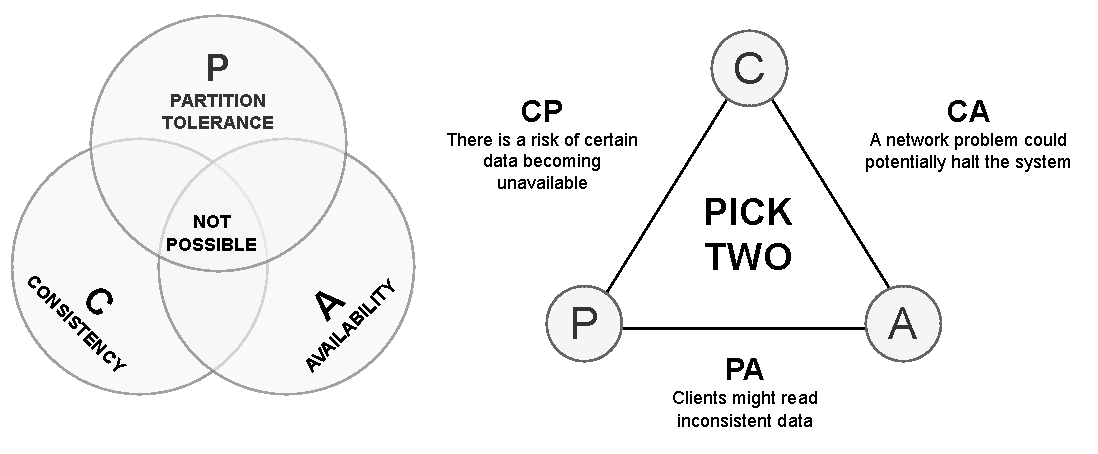
\includegraphics[width=\linewidth]{introduction/cap-theorem.pdf}
    \caption{CAP Theorem}
    \label{fig:cap-theorem}
\end{figure}

Moreover, there has been a trend towards the adoption of asynchronous patterns utilizing event streaming processing such as Apache Kafka.
These platforms are utilized to collect, store and process events representing asynchronous operations that lack a discrete beginning or end.

The Figure \ref{fig:cloud-architecture} illustrates a commonly employed cloud architecture. Clients undergo authentication with a centralized Identity Provider, which subsequently issues a token to the client.
The client then uses this token to access the resources of the server.
Two widely embraced protocols in this context are OpenID \cite{c4} and OAuth \cite{c5}. OpenID serves as an open standard for authentication, while OAuth functions as an open standard for authorization.

\begin{figure*}[htbp]
    \centering
    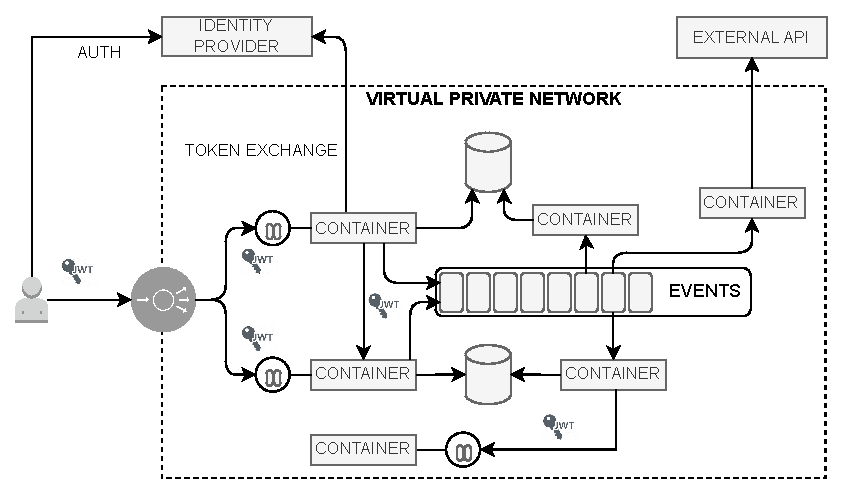
\includegraphics[width=0.7\textwidth]{introduction/cloud-architecture.pdf}
    \caption{Cloud Architecture}
    \label{fig:cloud-architecture}
\end{figure*}

Within the scope of these protocols, JSON Web Token (JWT) \cite{c6} has gained notable significance. JWT offers a concise and URL-safe approach for exchanging claims between two parties.
These tokens are encoded and digitally signed, enhancing their integrity and ensuring secure communication between the server and the client.
Additionally, this token format streamlines and enhances the efficiency of verification, thereby contributing to the overall security and reliability of the authentication and authorization mechanisms in cloud-based systems.

Among these software solutions, access control stands out as a critical aspect. Models like Role-Based Access Control (RBAC) and Annotation-Based Access Control (ABAC) contribute to the rise of Policy-Based Access Control (PBAC) \cite{c7}

PBAC, or Policy-Based Access Control, is a method for managing system access control through dynamic policies. Instead of relying on permissions granted by static roles, PBAC employs rules and conditions to determine who can access specific resources. 
It offers a flexible approach, enabling organizations to customize access control based on specific needs. PBAC is recognized for its adaptability and capability to accommodate complex access requirements in diverse system environments.

PBAC policies must be linked to identities, where identities encompass users, and roles. However, this approach currently lacks standardization and exposes systems to various security threats.
Therefore, the scope of this paper is to propose a standardized PBAC approach.

The primary consideration is that the Access Control layer should not be embedded within the software solution; instead, it should be provided as an external Access Control Solution (ACS). 
The main reason relies on the fact that Access Control is a software aspect that is too complex and error-prone to be implemented in each individual software solution.
Ideally, the ACS should support the creation of separate accounts, enabling each organization to manage the access control of its software solutions within one or more isolated accounts as per Figure \ref{fig:accounts}.

The ACS can be seen as a platform that enables organizations to create one or more accounts for modeling Access Control. Additionally, it must support the federation of these accounts to enable cross-account access control management when needed.

Taking a closer look, let's break down the following concepts for the ACS:

\begin{figure}[ht]
    \centering
    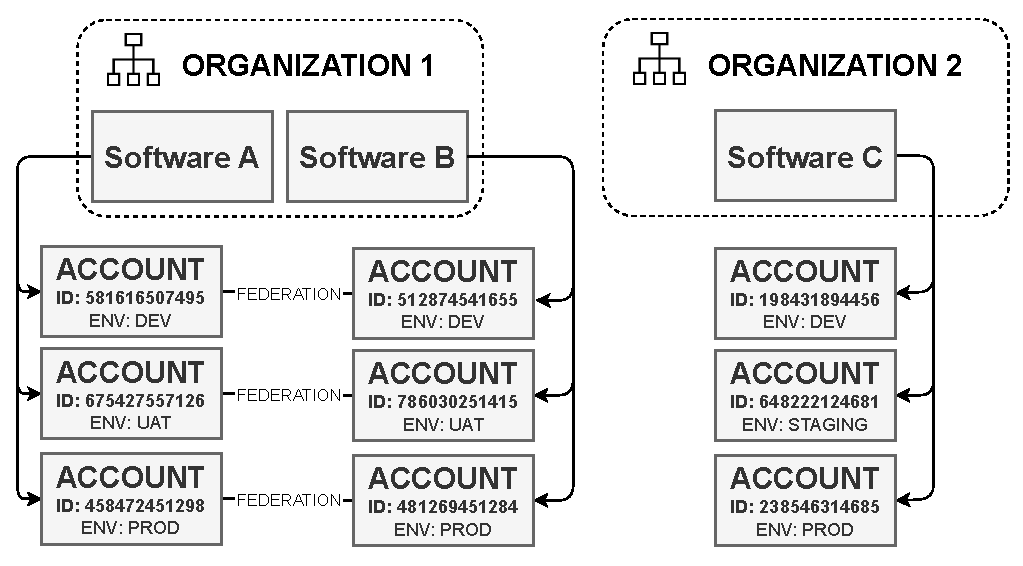
\includegraphics[width=\linewidth]{introduction/accounts.pdf}
    \caption{Accounts}
    \label{fig:accounts}
\end{figure}

\begin{itemize}
    \item \textbf{Account}: An account is the top-level entity in the hierarchy used for managing environment and systems isolation and configurations. It is identified by an AccountId and is associated with a single email address.
    \item \textbf{Identity}: The system can be accessed through identities, taking the form of Users, and Roles. In this context, a Principal is either a human user or a workload with granted permissions, responsible for authentication and initiating requests.
    \item \textbf{Tenant}: A tenant is an entity that accesses specific resources within an account. Ownership of resources can be divided or shared among tenants, and multiple identities can be associated with a tenant.
    \item \textbf{Project}: An account can be partitioned into projects, where each project represents a system.
    \item \textbf{Domain}: A project can be segmented into multiple domains using preferred techniques such as Domain-Driven Design (DDD), with at least one domain necessary for each project.
    \item \textbf{Resource}: Resources in a domain represent domain entities. While they may not directly align with system entities, they indicate logical resources crucial for defining access control policies.
    \item \textbf{Action}: Actions are operations that affect the state of resources.
    \item \textbf{Policy}: A policy is a collection of predefined rules evaluated to determine if a specific identity has been granted the right to perform a certain action.
\end{itemize}

The paper aims to formalize an approach using relational structures, relational algebra, and operations. Additionally, it seeks to implement risk scores generation approach to help mitigate security risks.

This paper is organized as follows: In the next section (\ref{sec:problemdefinition}), the identified and defined problems are discussed. Section \ref{sec:permissioningapproach} outlines the proposed approach, followed by Section \ref{sec:generatedriskscores}, where the generation of risk scores approach is introduced. Finally, Section \ref{sec:conclusion} discusses the conclusions.
